\documentclass[aspectratio=169, 10pt]{beamer}
\usepackage[utf8]{inputenc}
\usepackage[T1]{fontenc}
\usepackage{helvet}
\usepackage{tikz}
\usepackage[most]{tcolorbox}
\usepackage{pgfplots}
\usepackage{booktabs}
\usepackage{multicol}
\usepackage{array}
\usepackage{tabularx}
\usepackage{fontawesome5}

\usetikzlibrary{shapes.geometric, arrows.meta, positioning, calc, shadows, fit, backgrounds}

\pgfplotsset{compat=1.18}

% Custom Enterprise Palette (Light Theme Only)
\definecolor{PrimaryColor}{HTML}{2563EB}
\definecolor{SecondaryColor}{HTML}{1E293B}
\definecolor{AccentColor}{HTML}{0EA5E9}
\definecolor{SuccessColor}{HTML}{10B981}
\definecolor{WarningColor}{HTML}{F59E0B}
\definecolor{BgColor}{HTML}{FFFFFF}
\definecolor{CardBg}{HTML}{F8FAFC}
\definecolor{CardBorder}{HTML}{CBD5E1}
\definecolor{TextDark}{HTML}{1E293B}
\definecolor{TextLight}{HTML}{64748B}

% Configure Beamer Custom Styling
\setbeamertemplate{navigation symbols}{}
\setbeamercolor{title}{fg=PrimaryColor}
\setbeamercolor{frametitle}{fg=SecondaryColor}
\setbeamercolor{structure}{fg=PrimaryColor}
\setbeamercolor{normal text}{fg=TextDark}
\setbeamercolor{background canvas}{bg=BgColor}

\setbeamertemplate{headline}{}

\setbeamertemplate{frametitle}{
  \vspace{3mm}
  \hspace{1mm}
  \begin{minipage}{0.95\paperwidth}
    \raggedright
    {\usebeamerfont{frametitle}\bfseries\color{SecondaryColor}\insertframetitle}
    \par\vspace{1mm}
    {\color{AccentColor}\hrule height 1pt}
  \end{minipage}
  \vspace{-1mm}
}

\setbeamertemplate{footline}{
  \begin{minipage}{\paperwidth}
    \color{CardBorder}\hrule height 0.5pt
    \vspace{2mm}
    \hspace{5mm}
    \color{TextLight}\scriptsize\sffamily
    Startup Ecosystem Analytics Platform \hfill DevOps \& Solution Architecture \hfill Slide \insertframenumber\ / \inserttotalframenumber
    \hspace{5mm}
    \vspace{2mm}
  \end{minipage}
}

\setbeamertemplate{title page}{
  \begin{tikzpicture}[remember picture, overlay]
    \fill[color=CardBg] (current page.south west) rectangle (current page.north east);
    
    % Geometric accent background
    \fill[color=PrimaryColor] (current page.north west) -- ($(current page.north west)+(4cm,0)$) -- ($(current page.south west)+(1.5cm,0)$) -- (current page.south west) -- cycle;
    \fill[color=AccentColor] ($(current page.north west)+(4cm,0)$) -- ($(current page.north west)+(4.3cm,0)$) -- ($(current page.south west)+(1.8cm,0)$) -- ($(current page.south west)+(1.5cm,0)$) -- cycle;
    
    \node[anchor=north west, text width=11cm, align=left] at ($(current page.north west)+(3.4cm,-1.2cm)$) {
      {\Huge\bfseries\color{SecondaryColor} Startup Ecosystem}\\[2.5mm]
      {\Large\bfseries\color{PrimaryColor} Analytics Platform}
    };

    \node[anchor=north west, draw=PrimaryColor!20, line width=1pt, fill=white, rounded corners=6pt,
          text width=8.5cm, inner sep=8pt, align=left] at ($(current page.north west)+(3.4cm,-3.6cm)$) {
      {\normalsize\bfseries\color{PrimaryColor} Team Members}\\[2mm]
      {\color{TextDark}\sffamily\small
        \begin{tabular}{@{}ll@{}}
          Srijan C Vachadmath & USN 1BM23CD060 \\
          Manohara Salmani & USN 1BM23CD035 \\
          Shreejth Shah & USN 1BM23CD057
        \end{tabular}
      }
    };

    \node[anchor=south west, text width=10.5cm, align=left] at ($(current page.south west)+(3.4cm,0.8cm)$) {
      {\scriptsize\color{TextLight}\sffamily Department of Computer Science and Engineering}
    };
  \end{tikzpicture}
}

% Reusable TColorBox Panels
\newtcolorbox{scard}[2][]{
  colback=CardBg,
  colframe=CardBorder,
  coltitle=BgColor,
  fonttitle=\bfseries\sffamily\scriptsize,
  colbacktitle=PrimaryColor,
  enhanced,
  boxrule=0.5pt,
  sharp corners,
  title={#2},
  attach boxed title to top left={yshift=-1.8mm, xshift=2.5mm},
  boxed title style={sharp corners, boxrule=0pt, top=0.8mm, bottom=0.8mm, left=2mm, right=2mm},
  top=3mm,
  bottom=2mm,
  left=2.5mm,
  right=2.5mm,
  fontupper=\sffamily\footnotesize,
  #1
}

\newtcolorbox{infobox}[2][]{
  colback=CardBg,
  colframe=PrimaryColor!20,
  leftrule=3.5pt,
  rightrule=0pt,
  toprule=0pt,
  bottomrule=0pt,
  sharp corners,
  boxrule=0.5pt,
  fonttitle=\bfseries\sffamily\footnotesize\color{PrimaryColor},
  title={#2},
  top=1.2mm,
  bottom=1.2mm,
  left=2mm,
  right=2mm,
  fontupper=\sffamily\footnotesize,
  #1
}

\newtcolorbox{successbox}[2][]{
  colback=SuccessColor!5,
  colframe=SuccessColor!20,
  leftrule=3.5pt,
  rightrule=0pt,
  toprule=0pt,
  bottomrule=0pt,
  sharp corners,
  boxrule=0.5pt,
  fonttitle=\bfseries\sffamily\footnotesize\color{SuccessColor},
  title={#2},
  top=1.2mm,
  bottom=1.2mm,
  left=2mm,
  right=2mm,
  fontupper=\sffamily\footnotesize,
  #1
}

\begin{document}

% Slide 1: Title Slide
\begin{frame}[plain]
  \titlepage
\end{frame}

% Slide 2: Problem Statement
\begin{frame}{Problem Statement}
  \begin{columns}[T]
    \begin{column}{0.48\textwidth}
      \begin{scard}{Relational DB Bottleneck}
        \begin{itemize}\setlength{\itemsep}{0.5pt}
          \item Multi-hop lookups (e.g., co-investments) require complex recursive SQL JOINs.
          \item Query latencies degrade exponentially under deep traversals.
        \end{itemize}
      \end{scard}
      \vspace{0.8mm}
      \begin{scard}{Concurrency \& Oversubscription}
        \begin{itemize}\setlength{\itemsep}{0.5pt}
          \item Concurrent funding calls read stale state, causing oversubscribed rounds.
          \item Lacks a thread-safe distributed lock manager.
        \end{itemize}
      \end{scard}
    \end{column}
    \begin{column}{0.48\textwidth}
      \begin{scard}{Unverified Data Lifecycles}
        \begin{itemize}\setlength{\itemsep}{0.5pt}
          \item Founders self-report accomplishments without third-party validation.
          \item No audit trail for investor due diligence.
        \end{itemize}
      \end{scard}
      \vspace{0.8mm}
      \begin{scard}{Blocking API Execution}
        \begin{itemize}\setlength{\itemsep}{0.5pt}
          \item Matchmaking queries block synchronous request loops.
          \item Real-time leaderboards and analytics cause UI lag under load.
        \end{itemize}
      \end{scard}
    \end{column}
  \end{columns}
\end{frame}

% Slide 3: Project Vision
\begin{frame}{Project Vision \& Solution Overview}
  \begin{columns}[T]
    \begin{column}{0.48\textwidth}
      \begin{scard}{Platform Objective}
        High-performance startup analytics platform mapping founders, startups, and investors.
        \begin{itemize}\setlength{\itemsep}{0.5pt}
          \item \textbf{Graph Topology:} Native property graph stores nodes/edges directly.
          \item \textbf{Sub-15ms Matching:} Hybrid ranking computed in DB memory.
        \end{itemize}
      \end{scard}
    \end{column}
    \begin{column}{0.48\textwidth}
      \begin{scard}{Multi-Role Portals}
        \begin{itemize}\setlength{\itemsep}{0.5pt}
          \item \textbf{Startups:} Manage asks, post achievements, accept interest.
          \item \textbf{Investors:} Set ticket bounds, check matches, transfer funds.
          \item \textbf{Analysts:} Verify milestones, top up wallets, inspect paths.
        \end{itemize}
      \end{scard}
    \end{column}
  \end{columns}
  \vspace{1.0mm}
  \begin{successbox}{Unified Value Proposition}
    Async FastAPI + Neo4j Graph + Redis cache \& mutex = Scalable, secure startup directory.
  \end{successbox}
\end{frame}

% Slide 4: Database Decision: Neo4j
\begin{frame}{Why Neo4j? — Graph Database Choice}
  \begin{columns}[T]
    \begin{column}{0.55\textwidth}
      \centering
      \footnotesize
      \begin{tabularx}{\textwidth}{lXX}
        \toprule
        \textbf{Metric} & \textbf{Neo4j 5.13} & \textbf{Traditional SQL} \\
        \midrule
        Traversals & Index-free adjacency & Recursive JOINs \\
        Edge Props & Native properties & Assoc. entities \\
        Flexibility & Schemaless labels & Rigid DDL migrations \\
        Path query & Bolt ($<$2ms) & Multi-query loops \\
        \bottomrule
      \end{tabularx}
      \vspace{1.5mm}
      \begin{infobox}{Connection Integrity}
        FastAPI lifespan configures persistent connection pool to \texttt{bolt://neo4j:7687} via Neo4j python driver, using autocommit and transactional queries.
      \end{infobox}
    \end{column}
    \begin{column}{0.42\textwidth}
      \begin{scard}{Use Case Rationale}
        \begin{itemize}\setlength{\itemsep}{0.5pt}
          \item \textbf{Natural Structure:} Startup ecosystem is inherently relational. Connecting founders, startups, and investors via physical links.
          \item \textbf{Traversal Speed:} Evaluates path matching queries recursively in microseconds.
        \end{itemize}
      \end{scard}
    \end{column}
  \end{columns}
\end{frame}

% Slide 5: Database Decision: Redis
\begin{frame}{Why Redis? — High-Performance Caching}
  \begin{columns}[T]
    \begin{column}{0.55\textwidth}
      \centering
      \footnotesize
      \begin{tabularx}{\textwidth}{lXX}
        \toprule
        \textbf{Feature} & \textbf{With Redis} & \textbf{Without Redis} \\
        \midrule
        Feed queries & Cached hit ($<$2ms) & DB query scan (50ms) \\
        Match lists & TTL-based lookup & On-the-fly math loop \\
        Round locks & Atomic lease (SET NX) & DB lock contention \\
        Leaderboards & ZSET sorted list & Aggregated group-by \\
        \bottomrule
      \end{tabularx}
      \vspace{1.5mm}
      \begin{infobox}{Revocation Control}
        JWT token IDs (JTI) blacklisted in Redis on logout for remaining token lifetime to enforce instant backend access revocation.
      \end{infobox}
    \end{column}
    \begin{column}{0.42\textwidth}
      \begin{scard}{Caching Strategy}
        \begin{itemize}\setlength{\itemsep}{0.5pt}
          \item \textbf{MD5 Hash Keys:} Keyed by query params, e.g. \texttt{feed:filtered:\{md5\}}.
          \item \textbf{Write Invalidation:} Mutations to profiles trigger immediate key deletes.
          \item \textbf{Atomic Lock Lease:} Prevents race conditions during funds transfer.
        \end{itemize}
      \end{scard}
    \end{column}
  \end{columns}
\end{frame}

% Slide 6: Neo4j Schema \& Graph Design
\begin{frame}{Neo4j Schema \& Graph Design}
  \begin{columns}[T]
    \begin{column}{0.60\textwidth}
      \centering
      \resizebox{!}{0.65\textheight}{
      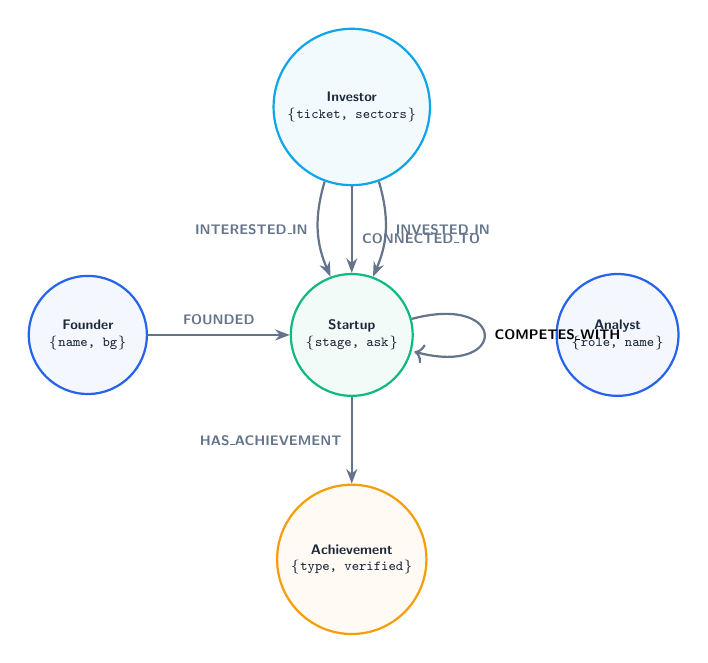
\begin{tikzpicture}[
        node distance=1.1cm and 1.8cm,
        gn/.style={circle, draw=PrimaryColor, fill=PrimaryColor!5, thick, minimum size=1.5cm, align=center, font=\sffamily\tiny\bfseries, text=TextDark},
        sn/.style={gn, draw=SuccessColor, fill=SuccessColor!5},
        invn/.style={gn, draw=AccentColor, fill=AccentColor!5},
        achn/.style={gn, draw=WarningColor, fill=WarningColor!5},
        arrow/.style={-{Stealth[scale=0.8]}, thick, TextLight, font=\sffamily\tiny\bfseries}
      ]
        % Nodes
        \node[gn] (founder) {Founder \\ \texttt{\{name, bg\}}};
        \node[sn, right=of founder] (startup) {Startup \\ \texttt{\{stage, ask\}}};
        \node[invn, above=of startup] (investor) {Investor \\ \texttt{\{ticket, sectors\}}};
        \node[achn, below=of startup] (achievement) {Achievement \\ \texttt{\{type, verified\}}};
        \node[gn, right=of startup] (analyst) {Analyst \\ \texttt{\{role, name\}}};

        % Edges
        \draw[arrow] (founder) -- node[above] {FOUNDED} (startup);
        \draw[arrow] (investor) to[bend left=20] node[right] {INVESTED\_IN} (startup);
        \draw[arrow] (investor) to[bend right=20] node[left] {INTERESTED\_IN} (startup);
        \draw[arrow] (investor) -- node[right, pos=0.6] {CONNECTED\_TO} (startup);
        \draw[arrow] (startup) -- node[left] {HAS\_ACHIEVEMENT} (achievement);
        \path (startup) edge[loop right, thick, draw=TextLight, Stealth-] node[right, font=\tiny\sffamily\bfseries] {COMPETES\_WITH} (startup);
      \end{tikzpicture}
      }
    \end{column}
    \begin{column}{0.37\textwidth}
      \begin{scard}{Entity Constraints}
        \begin{itemize}\setlength{\itemsep}{0.5pt}
          \item Uniqueness constraint on \texttt{Startup.id}.
          \item Uniqueness constraint on \texttt{Investor.id}.
          \item Property indexes on sector and stage attributes.
        \end{itemize}
      \end{scard}
    \end{column}
  \end{columns}
\end{frame}

% Slide 7: Redis Implementation
\begin{frame}{Redis Architecture \& Data Flow}
  \begin{columns}[T]
    \begin{column}{0.65\textwidth}
      \centering
      \resizebox{\textwidth}{!}{
      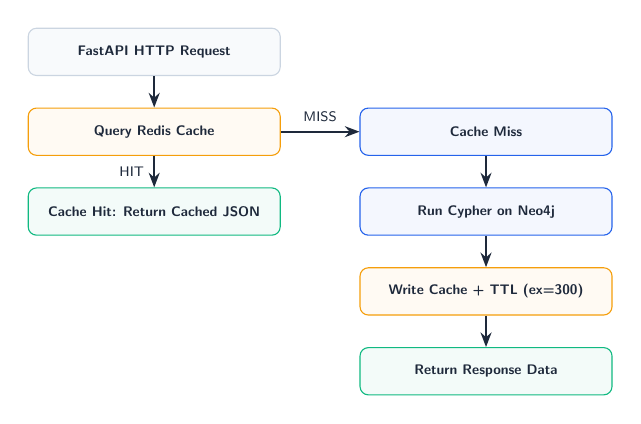
\begin{tikzpicture}[
        node distance=0.4cm and 1.0cm,
        box/.style={rectangle, draw=CardBorder, fill=CardBg, rounded corners=3pt, minimum width=3.2cm, minimum height=0.6cm, align=center, font=\sffamily\tiny\bfseries, text=TextDark},
        rbox/.style={box, draw=WarningColor, fill=WarningColor!5},
        dbox/.style={box, draw=PrimaryColor, fill=PrimaryColor!5},
        sbox/.style={box, draw=SuccessColor, fill=SuccessColor!5},
        arr/.style={-{Stealth[scale=0.8]}, thick, SecondaryColor}
      ]
        \node[box] (req) {FastAPI HTTP Request};
        \node[rbox, below=of req] (chk) {Query Redis Cache};
        \node[sbox, below=of chk] (hit) {Cache Hit: Return Cached JSON};
        \node[dbox, right=of chk] (miss) {Cache Miss};
        \node[dbox, below=of miss] (neo) {Run Cypher on Neo4j};
        \node[rbox, below=of neo] (set) {Write Cache + TTL (ex=300)};
        \node[sbox, below=of set] (resp) {Return Response Data};

        \draw[arr] (req) -- (chk);
        \draw[arr] (chk) -- node[left, font=\tiny\sffamily] {HIT} (hit);
        \draw[arr] (chk) -- node[above, font=\tiny\sffamily] {MISS} (miss);
        \draw[arr] (miss) -- (neo);
        \draw[arr] (neo) -- (set);
        \draw[arr] (set) -- (resp);
      \end{tikzpicture}
      }
    \end{column}
    \begin{column}{0.32\textwidth}
      \begin{scard}{Storage Details}
        \begin{itemize}\setlength{\itemsep}{0.5pt}
          \item \textbf{Hashes:} \texttt{views:startup:\{id\}} stores viewer metadata.
          \item \textbf{Sorted Sets:} \texttt{leaderboard:investors} rankings.
          \item \textbf{Strings:} JSON cached payload with explicit expiration.
        \end{itemize}
      \end{scard}
    \end{column}
  \end{columns}
\end{frame}

% Slide 8: High Level Architecture
\begin{frame}{System Architecture Overview}
  \begin{columns}[T]
    \begin{column}{0.65\textwidth}
      \centering
      \resizebox{\textwidth}{!}{
      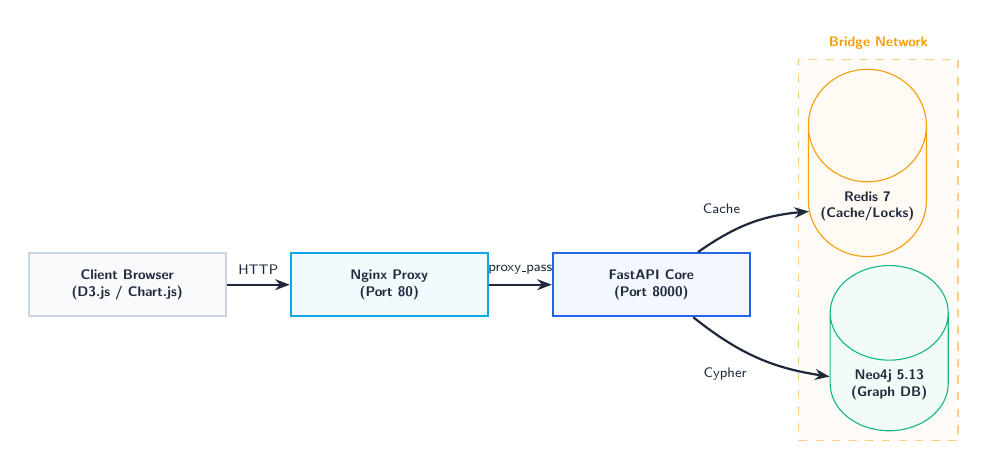
\begin{tikzpicture}[
        node distance=0.8cm and 0.8cm,
        box/.style={rectangle, draw=CardBorder, fill=CardBg, thick, minimum width=2.5cm, minimum height=0.8cm, align=center, font=\sffamily\tiny\bfseries, text=TextDark},
        primarybox/.style={box, draw=PrimaryColor, fill=PrimaryColor!5, minimum width=2.5cm},
        accentbox/.style={box, draw=AccentColor, fill=AccentColor!5},
        dbbox/.style={cylinder, draw=SecondaryColor, fill=SecondaryColor!5, shape border rotate=90, minimum width=1.5cm, minimum height=1.0cm, align=center, font=\sffamily\tiny\bfseries, text=TextDark},
        arrow/.style={-{Stealth[scale=0.8]}, thick, SecondaryColor}
      ]
        % Nodes
        \node[box] (browser) {Client Browser \\ (D3.js / Chart.js)};
        \node[accentbox, right=of browser] (nginx) {Nginx Proxy \\ (Port 80)};
        \node[primarybox, right=of nginx] (fastapi) {FastAPI Core \\ (Port 8000)};
        \node[dbbox, draw=WarningColor, fill=WarningColor!5, above right=0.1cm and 1.0cm of fastapi] (redis) {Redis 7 \\ (Cache/Locks)};
        \node[dbbox, draw=SuccessColor, fill=SuccessColor!5, below right=0.1cm and 1.0cm of fastapi] (neo4j) {Neo4j 5.13 \\ (Graph DB)};

        % Connections
        \draw[arrow] (browser) -- node[above, font=\tiny\sffamily] {HTTP} (nginx);
        \draw[arrow] (nginx) -- node[above, font=\tiny\sffamily] {proxy\_pass} (fastapi);
        \draw[arrow] (fastapi) to[bend left=15] node[above left, font=\tiny\sffamily] {Cache} (redis);
        \draw[arrow] (fastapi) to[bend right=15] node[below left, font=\tiny\sffamily] {Cypher} (neo4j);
        
        \begin{scope}[on background layer]
          \node[draw=WarningColor!50, fill=WarningColor!3, dashed, fit=(redis) (neo4j), label={[font=\tiny\sffamily\bfseries, WarningColor]above:Bridge Network}] (dbGroup) {};
        \end{scope}
      \end{tikzpicture}
      }
    \end{column}
    \begin{column}{0.32\textwidth}
      \begin{scard}{Gateway Security}
        \begin{itemize}\setlength{\itemsep}{0.5pt}
          \item Nginx exposes Port 80 and reverse proxies downstream.
          \item Restricts DB Bolt/Redis ports to private virtual bridge.
        \end{itemize}
      \end{scard}
    \end{column}
  \end{columns}
\end{frame}

% Slide 9: Startup User Journey
\begin{frame}{Startup User Journey}
  \begin{columns}[T]
    \begin{column}{0.54\textwidth}
      \centering
      \resizebox{!}{0.65\textheight}{
      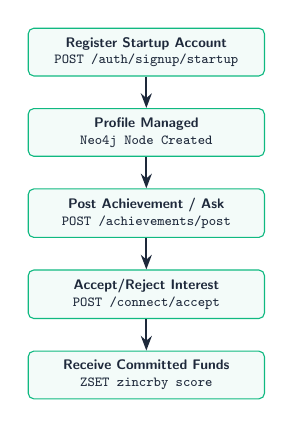
\begin{tikzpicture}[
        node distance=0.4cm and 0.8cm,
        sstep/.style={rectangle, draw=SuccessColor, fill=SuccessColor!5, rounded corners=2pt, minimum width=3.0cm, minimum height=0.6cm, align=center, font=\sffamily\tiny\bfseries, text=TextDark},
        arr/.style={-{Stealth[scale=0.8]}, thick, SecondaryColor}
      ]
        \node[sstep] (reg) {Register Startup Account \\ \texttt{POST /auth/signup/startup}};
        \node[sstep, below=of reg] (prof) {Profile Managed \\ \texttt{Neo4j Node Created}};
        \node[sstep, below=of prof] (ach) {Post Achievement / Ask \\ \texttt{POST /achievements/post}};
        \node[sstep, below=of ach] (dec) {Accept/Reject Interest \\ \texttt{POST /connect/accept}};
        \node[sstep, below=of dec] (fund) {Receive Committed Funds \\ \texttt{ZSET zincrby score}};

        \draw[arr] (reg) -- (prof);
        \draw[arr] (prof) -- (ach);
        \draw[arr] (ach) -- (dec);
        \draw[arr] (dec) -- (fund);
      \end{tikzpicture}
      }
    \end{column}
    \begin{column}{0.42\textwidth}
      \begin{scard}{Key Workflow States}
        \begin{itemize}\setlength{\itemsep}{0.5pt}
          \item \textbf{Unverified posts:} Post achievements which go into the queue.
          \item \textbf{Match feed:} Retrieve matched investors based on scoring.
        \end{itemize}
      \end{scard}
    \end{column}
  \end{columns}
\end{frame}

% Slide 10: Investor User Journey
\begin{frame}{Investor User Journey}
  \begin{columns}[T]
    \begin{column}{0.54\textwidth}
      \centering
      \resizebox{!}{0.65\textheight}{
      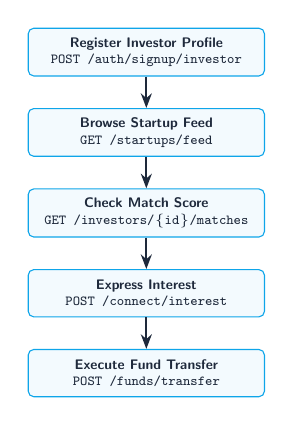
\begin{tikzpicture}[
        node distance=0.4cm and 0.8cm,
        istep/.style={rectangle, draw=AccentColor, fill=AccentColor!5, rounded corners=2pt, minimum width=3.0cm, minimum height=0.6cm, align=center, font=\sffamily\tiny\bfseries, text=TextDark},
        arr/.style={-{Stealth[scale=0.8]}, thick, SecondaryColor}
      ]
        \node[istep] (reg) {Register Investor Profile \\ \texttt{POST /auth/signup/investor}};
        \node[istep, below=of reg] (browse) {Browse Startup Feed \\ \texttt{GET /startups/feed}};
        \node[istep, below=of browse] (match) {Check Match Score \\ \texttt{GET /investors/\{id\}/matches}};
        \node[istep, below=of match] (interest) {Express Interest \\ \texttt{POST /connect/interest}};
        \node[istep, below=of interest] (transfer) {Execute Fund Transfer \\ \texttt{POST /funds/transfer}};

        \draw[arr] (reg) -- (browse);
        \draw[arr] (browse) -- (match);
        \draw[arr] (match) -- (interest);
        \draw[arr] (interest) -- (transfer);
      \end{tikzpicture}
      }
    \end{column}
    \begin{column}{0.42\textwidth}
      \begin{scard}{Financial Pipeline}
        \begin{itemize}\setlength{\itemsep}{0.5pt}
          \item \textbf{Initial Capital:} Given \$500,000 wallet balance on signup.
          \item \textbf{Validation:} Asks cannot exceed available balance.
        \end{itemize}
      \end{scard}
    \end{column}
  \end{columns}
\end{frame}

% Slide 11: Analyst User Journey
\begin{frame}{Analyst User Journey}
  \begin{columns}[T]
    \begin{column}{0.54\textwidth}
      \centering
      \resizebox{!}{0.65\textheight}{
      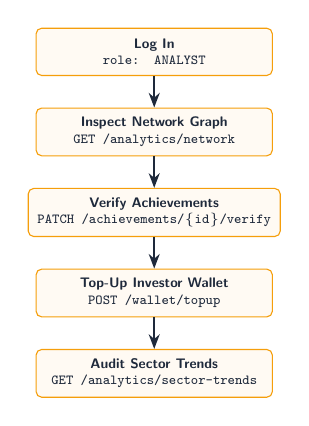
\begin{tikzpicture}[
        node distance=0.4cm and 0.8cm,
        astep/.style={rectangle, draw=WarningColor, fill=WarningColor!5, rounded corners=2pt, minimum width=3.0cm, minimum height=0.6cm, align=center, font=\sffamily\tiny\bfseries, text=TextDark},
        arr/.style={-{Stealth[scale=0.8]}, thick, SecondaryColor}
      ]
        \node[astep] (login) {Log In \\ \texttt{role: ANALYST}};
        \node[astep, below=of login] (net) {Inspect Network Graph \\ \texttt{GET /analytics/network}};
        \node[astep, below=of net] (ver) {Verify Achievements \\ \texttt{PATCH /achievements/\{id\}/verify}};
        \node[astep, below=of ver] (top) {Top-Up Investor Wallet \\ \texttt{POST /wallet/topup}};
        \node[astep, below=of top] (trend) {Audit Sector Trends \\ \texttt{GET /analytics/sector-trends}};

        \draw[arr] (login) -- (net);
        \draw[arr] (net) -- (ver);
        \draw[arr] (ver) -- (top);
        \draw[arr] (top) -- (trend);
      \end{tikzpicture}
      }
    \end{column}
    \begin{column}{0.42\textwidth}
      \begin{scard}{Analytics Tools}
        \begin{itemize}\setlength{\itemsep}{0.5pt}
          \item \textbf{Global view:} Displays co-investments and connections across the entire system.
          \item \textbf{Authority Actions:} Verifies startup achievements to update matches.
        \end{itemize}
      \end{scard}
    \end{column}
  \end{columns}
\end{frame}

% Slide 12: DevOps Toolstack
\begin{frame}{DevOps \& Infrastructure Stack}
  \begin{columns}[T]
    \begin{column}{0.48\textwidth}
      \begin{scard}{Code \& Build Automation}
        \begin{itemize}\setlength{\itemsep}{0pt}
          \item \textbf{Git / GitHub:} Hosts source code and manifests.
          \item \textbf{Jenkins CI/CD:} 6-stage pipeline in \texttt{Jenkinsfile}.
          \item \textbf{GitHub Actions:} PR workflow validating code syntax.
        \end{itemize}
      \end{scard}
      \vspace{0.5mm}
      \begin{scard}{Virtualization \& Runtime}
        \begin{itemize}\setlength{\itemsep}{0pt}
          \item \textbf{Docker Containers:} Multi-stage builds for backend and frontend.
          \item \textbf{Docker Compose:} Configures isolated networks and volumes.
        \end{itemize}
      \end{scard}
    \end{column}
    \begin{column}{0.48\textwidth}
      \begin{scard}{Serving \& Storage}
        \begin{itemize}\setlength{\itemsep}{0pt}
          \item \textbf{Nginx:} Proxy for static and dynamic endpoints.
          \item \textbf{Neo4j \& Redis:} Property graph database and in-memory key-value cache.
          \item \textbf{Pytest Testing:} Boundary verification testing.
        \end{itemize}
      \end{scard}
    \end{column}
  \end{columns}
\end{frame}

% Slide 13: Docker & Containerization
\begin{frame}{Containerization Strategy}
  \begin{columns}[T]
    \begin{column}{0.65\textwidth}
      \centering
      \resizebox{\textwidth}{!}{
      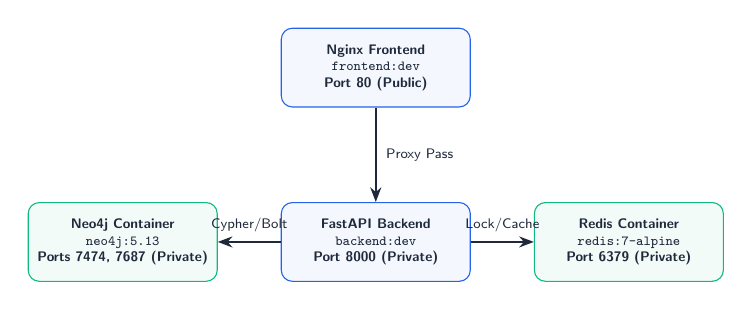
\begin{tikzpicture}[
        node distance=0.4cm and 0.8cm,
        cont/.style={rectangle, draw=PrimaryColor, fill=PrimaryColor!5, rounded corners=4pt, minimum width=2.4cm, minimum height=1.0cm, align=center, font=\sffamily\tiny\bfseries, text=TextDark},
        pub/.style={cont, draw=SuccessColor, fill=SuccessColor!5},
        arr/.style={-{Stealth[scale=0.8]}, thick, SecondaryColor}
      ]
        \node[cont] (nginx) {Nginx Frontend \\ \texttt{frontend:dev} \\ Port 80 (Public)};
        \node[cont, below=1.2cm of nginx] (backend) {FastAPI Backend \\ \texttt{backend:dev} \\ Port 8000 (Private)};
        \node[pub, right=of backend] (redis) {Redis Container \\ \texttt{redis:7-alpine} \\ Port 6379 (Private)};
        \node[pub, left=of backend] (neo4j) {Neo4j Container \\ \texttt{neo4j:5.13} \\ Ports 7474, 7687 (Private)};

        \draw[arr] (nginx) -- node[right, font=\tiny\sffamily] {Proxy Pass} (backend);
        \draw[arr] (backend) -- node[above, font=\tiny\sffamily] {Lock/Cache} (redis);
        \draw[arr] (backend) -- node[above, font=\tiny\sffamily] {Cypher/Bolt} (neo4j);
      \end{tikzpicture}
      }
    \end{column}
    \begin{column}{0.32\textwidth}
      \begin{scard}{Isolation Model}
        \begin{itemize}
          \item Backend runs on a lightweight Debian-slim base image.
          \item Only Nginx binds to host Port 80, shielding API servers.
          \item Neo4j data folders mapped to persistent docker volumes.
        \end{itemize}
      \end{scard}
    \end{column}
  \end{columns}
\end{frame}

% Slide 14: Jenkins CI/CD Pipeline
\begin{frame}{Jenkins Pipeline Implementation}
  \begin{columns}[T]
    \begin{column}{0.48\textwidth}
      \centering
      \resizebox{!}{0.65\textheight}{
      \begin{tikzpicture}[
        node distance=0.2cm and 0.8cm,
        stage/.style={rectangle, draw=PrimaryColor, fill=CardBg, rounded corners=3pt, minimum width=3.4cm, minimum height=0.55cm, align=center, font=\sffamily\tiny\bfseries, text=TextDark},
        arr/.style={-{Stealth[scale=0.8]}, thick, SecondaryColor}
      ]
        % Pipeline Nodes
        \node[stage] (checkout) {\faGit*~Checkout \\ Clones main branch};
        \node[stage, below=of checkout] (validate) {\faPython~Workspace \& Backend Audit \\ Lint \& Syntax Compiles};
        \node[stage, below=of validate] (build) {\faDocker~Docker Build \\ Builds frontend \& backend images};
        \node[stage, below=of build] (deploy) {\faServer~Docker Compose Stack \\ Up --force-recreate};
        \node[stage, below=of deploy] (health) {\faHeartbeat~Health Checks \\ Active Neo4j/Redis REST Probes};
        \node[stage, below=of health] (summary) {\faFile~Publish Results \\ Success/Failure Summary};

        % Transitions
        \draw[arr] (checkout) -- (validate);
        \draw[arr] (validate) -- (build);
        \draw[arr] (build) -- (deploy);
        \draw[arr] (deploy) -- (health);
        \draw[arr] (health) -- (summary);
      \end{tikzpicture}
      }
    \end{column}
    \begin{column}{0.48\textwidth}
      \begin{scard}{Safety Gates}
        \begin{itemize}\setlength{\itemsep}{0.5pt}
          \item Automatically cleans up orphan docker networks.
          \item Triggers rollback if backend port 8000 health pings fail.
          \item Seeds empty databases on deployment verify.
        \end{itemize}
      \end{scard}
    \end{column}
  \end{columns}
\end{frame}% Slide 15: CI/CD Workflow Lifecycle
\begin{frame}{CI/CD Workflow -- Startup Ecosystem Analytics Platform}
  \begin{columns}[T]
    \begin{column}{0.58\textwidth}
      \centering
      \resizebox{!}{0.50\textheight}{
      \begin{tikzpicture}[
        node distance=0.2cm and 0.6cm,
        wstep/.style={rectangle, draw=PrimaryColor, fill=CardBg, rounded corners=3pt, minimum width=2.7cm, minimum height=0.55cm, align=center, font=\sffamily\tiny\bfseries, text=TextDark},
        dev/.style={wstep, draw=AccentColor, fill=AccentColor!5},
        git/.style={wstep, draw=SecondaryColor, fill=SecondaryColor!5},
        jenk/.style={wstep, draw=PrimaryColor, fill=PrimaryColor!5},
        succ/.style={wstep, draw=SuccessColor, fill=SuccessColor!5},
        arr/.style={-{Stealth[scale=0.8]}, thick, SecondaryColor}
      ]
        % Left Column (Steps 1-5)
        \node[dev] (s1) {\faKeyboard~1. Developer Commit \\ \tiny\color{TextLight}\sffamily Code changes ready};
        \node[git, below=of s1] (s2) {\faGithub~2. GitHub Push \\ \tiny\color{TextLight}\sffamily Central repo update};
        \node[git, below=of s2] (s3) {\faLink~3. Webhook Trigger \\ \tiny\color{TextLight}\sffamily Notify Jenkins CI};
        \node[jenk, below=of s3] (s4) {\faCogs~4. Jenkins Execution \\ \tiny\color{TextLight}\sffamily Pipeline starts};
        \node[jenk, below=of s4] (s5) {\faGit*~5. Source Checkout \\ \tiny\color{TextLight}\sffamily Clones latest code};

        % Right Column (Steps 6-10)
        \node[jenk, right=1.0cm of s1] (s6) {\faClipboardCheck~6. Workspace Audit \\ \tiny\color{TextLight}\sffamily Validate python/docker};
        \node[jenk, below=of s6] (s7) {\faDocker~7. Docker Image Build \\ \tiny\color{TextLight}\sffamily Build app images};
        \node[jenk, below=of s7] (s8) {\faServer~8. Stack Deployment \\ \tiny\color{TextLight}\sffamily Docker Compose Up};
        \node[jenk, below=of s8] (s9) {\faHeartbeat~9. Health Verify \\ \tiny\color{TextLight}\sffamily API \& DB REST probes};
        \node[succ, below=of s9] (s10) {\faCheck~10. Success Staging \\ \tiny\color{TextLight}\sffamily Active deployment};

        % Connections
        \draw[arr] (s1) -- (s2);
        \draw[arr] (s2) -- (s3);
        \draw[arr] (s3) -- (s4);
        \draw[arr] (s4) -- (s5);
        \draw[arr] (s5.east) -- ++(0.5,0) |- (s6.west);
        \draw[arr] (s6) -- (s7);
        \draw[arr] (s7) -- (s8);
        \draw[arr] (s8) -- (s9);
        \draw[arr] (s9) -- (s10);
      \end{tikzpicture}
      }
    \end{column}
    \begin{column}{0.38\textwidth}
      \begin{scard}{CI/CD Pipeline Benefits}
        \begin{itemize}\setlength{\itemsep}{0pt}
          \item \textbf{Automation:} Commits trigger build/test automatically.
          \item \textbf{Mitigation:} Linting catches bugs before deploy.
          \item \textbf{Containers:} Images guarantee environment consistency.
          \item \textbf{Reliability:} Health checks and rollback.
        \end{itemize}
      \end{scard}
      \vspace{0.5mm}
      \begin{successbox}{Pipeline Efficiency}
        Reduces manual overhead and ensures stable releases.
      \end{successbox}
    \end{column}
  \end{columns}
\end{frame}

% Slide 16: CI/CD Workflow Overview & Benefits
\begin{frame}{CI/CD Workflow -- Overview \& Benefits}
  \begin{columns}[T]
    \begin{column}{0.48\textwidth}
      \begin{scard}{Platform Overview}
        Automated CI/CD workflow using GitHub, Jenkins, Docker, and Docker Compose.
        \begin{itemize}\setlength{\itemsep}{0.5pt}
          \item \textbf{Continuous Integration:} Pushes trigger Jenkins webhook pings.
          \item \textbf{Automated Testing:} Workspace is linted, compiled, and audited.
          \item \textbf{Virtualization:} Services are containerized into Docker images.
        \end{itemize}
      \end{scard}
      \vspace{0.5mm}
      \begin{infobox}{Automated Pipeline}
        Validates, containerizes, and deploys changes automatically to improve reliability.
      \end{infobox}
    \end{column}
    \begin{column}{0.48\textwidth}
      \begin{successbox}{Benefits of the CI/CD Pipeline}
        \begin{itemize}\setlength{\itemsep}{-1.0pt}
          \item[\faCheck] \textbf{Automated Builds:} Standardizes image creation.
          \item[\faCheck] \textbf{Auto Deployment:} Seamless stack updates.
          \item[\faCheck] \textbf{Early Detection:} Fails fast before production.
          \item[\faCheck] \textbf{Consistency:} Avoids configuration drift.
          \item[\faCheck] \textbf{Faster Releases:} Accelerates release iterations.
          \item[\faCheck] \textbf{High Reliability:} Solidifies continuous delivery.
          \item[\faCheck] \textbf{Seamless CI:} Integrates new features easily.
          \item[\faCheck] \textbf{Fewer Errors:} Removes manual mistakes.
        \end{itemize}
      \end{successbox}
    \end{column}
  \end{columns}
\end{frame}

% Slide 16: Other DevOps Tooling
\begin{frame}{Supporting Services \& Automation}
  \begin{columns}[T]
    \begin{column}{0.48\textwidth}
      \begin{scard}{Nginx Traffic Controller}
        \begin{itemize}
          \item Handles static HTML file delivery directly, bypassing Python thread pools.
          \item Proxies dynamic \texttt{/health} and auth endpoints directly to FastAPI.
          \item Inject reverse proxy headers including \texttt{X-Real-IP}.
        \end{itemize}
      \end{scard}
    \end{column}
    \begin{column}{0.48\textwidth}
      \begin{scard}{Environment Isolation}
        \begin{itemize}
          \item Configuration managed through isolated dotenv (\texttt{.env}) bindings.
          \item Enables easy transitions between dev ports and staging settings.
          \item Dynamic startup hooks run database index statements automatically.
        \end{itemize}
      \end{scard}
    \end{column}
  \end{columns}
\end{frame}

% Slide 16: API Architecture
\begin{frame}{API Architecture \& Route Schema}
  \begin{columns}[T]
    \begin{column}{0.5\textwidth}
      \begin{scard}{Core FastAPI Routers}
        \begin{itemize}
          \item \textbf{Startups:} \texttt{/startups/feed}, \texttt{/startups/register}, \texttt{/startups/\{id\}/matches}
          \item \textbf{Investors:} \texttt{/investors/register}, \texttt{/investors/\{id\}/matches}, \texttt{/investors/\{id\}/view/\{sid\}}
          \item \textbf{Funds:} \texttt{/funds/transfer}, \texttt{/funds/history/\{id\}}, \texttt{/wallet/topup}
          \item \textbf{Connections:} \texttt{/connect/interest}, \texttt{/connect/accept}, \texttt{/connect/reject}
          \item \textbf{Achievements:} \texttt{/achievements/post}, \texttt{/achievements/\{id\}/verify}
        \end{itemize}
      \end{scard}
    \end{column}
    \begin{column}{0.46\textwidth}
      \begin{scard}{Validation Pipeline}
        \begin{itemize}
          \item STRICT input checks via Pydantic schema models.
          \item \texttt{StartupCreate} \& \texttt{InvestorCreate} reject invalid email strings or weak passwords ($<$6 chars) at the request layer.
        \end{itemize}
      \end{scard}
    \end{column}
  \end{columns}
\end{frame}

% Slide 17: Security Architecture
\begin{frame}{Security Architecture \& Access Controls}
  \begin{columns}[T]
    \begin{column}{0.48\textwidth}
      \begin{scard}{HMAC Token Signing}
        \begin{itemize}
          \item Token payloads containing subject, name, role and unique JTI token ID are signed using HMAC-SHA256.
          \item Expired or malformed tokens raise an immediate \texttt{401 Unauthorized} code.
          \item Revocations validated via Redis token blacklist checking.
        \end{itemize}
      \end{scard}
    \end{column}
    \begin{column}{0.48\textwidth}
      \begin{scard}{Role Boundary Checks}
        \begin{itemize}
          \item Custom python decorators enforce role parameters per route.
          \item Parametrized Cypher query syntax prevents NoSQL injection attempts.
          \item Enforces secure password storage via salted bcrypt hashes.
        \end{itemize}
      \end{scard}
    \end{column}
  \end{columns}
\end{frame}

% Slide 18: Transaction Lock Lifecycle
\begin{frame}{Transaction Lock Lifecycle}
  \begin{columns}[T]
    \begin{column}{0.58\textwidth}
      \centering
      \resizebox{!}{0.65\textheight}{
      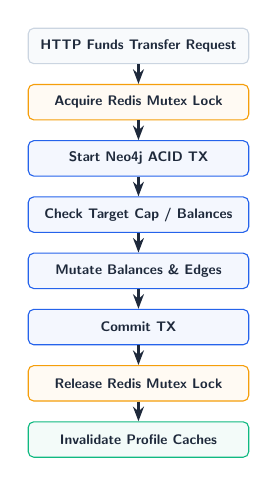
\begin{tikzpicture}[
        node distance=0.25cm and 0.8cm,
        box/.style={rectangle, draw=CardBorder, fill=CardBg, rounded corners=2pt, minimum width=2.8cm, minimum height=0.45cm, align=center, font=\sffamily\tiny\bfseries, text=TextDark},
        lock/.style={box, draw=WarningColor, fill=WarningColor!5},
        db/.style={box, draw=PrimaryColor, fill=PrimaryColor!5},
        success/.style={box, draw=SuccessColor, fill=SuccessColor!5},
        arr/.style={-{Stealth[scale=0.8]}, thick, SecondaryColor}
      ]
        % Nodes
        \node[box] (start) {HTTP Funds Transfer Request};
        \node[lock, below=of start] (acquire) {Acquire Redis Mutex Lock};
        \node[db, below=of acquire] (txstart) {Start Neo4j ACID TX};
        \node[db, below=of txstart] (check) {Check Target Cap / Balances};
        \node[db, below=of check] (write) {Mutate Balances \& Edges};
        \node[db, below=of write] (commit) {Commit TX};
        \node[lock, below=of commit] (release) {Release Redis Mutex Lock};
        \node[success, below=of release] (done) {Invalidate Profile Caches};

        % Connections
        \draw[arr] (start) -- (acquire);
        \draw[arr] (acquire) -- (txstart);
        \draw[arr] (txstart) -- (check);
        \draw[arr] (check) -- (write);
        \draw[arr] (write) -- (commit);
        \draw[arr] (commit) -- (release);
        \draw[arr] (release) -- (done);
      \end{tikzpicture}
      }
    \end{column}
    \begin{column}{0.38\textwidth}
      \begin{scard}{Protection Mechanics}
        \begin{itemize}\setlength{\itemsep}{0.5pt}
          \item Mutex lock uses a 10s auto-expiry.
          \item Rejects transactions if startup funding limit is exceeded.
          \item ZSET and cache invalidation run on success.
        \end{itemize}
      \end{scard}
    \end{column}
  \end{columns}
\end{frame}

% Slide 19: Pytest Testing Infrastructure
\begin{frame}{Pytest Testing \& Verification}
  \begin{columns}[T]
    \begin{column}{0.48\textwidth}
      \begin{scard}{Unit \& Mock Framework}
        \begin{itemize}
          \item Mock drivers simulate Neo4j endpoints and Redis pings in memory.
          \item Tests execute in isolation using GitHub Actions runner.
          \item Ensures database client failsafe boot modes work.
        \end{itemize}
      \end{scard}
    \end{column}
    \begin{column}{0.48\textwidth}
      \begin{scard}{Boundary Conditions Validated}
        \begin{itemize}
          \item Validates token signature tampering and expiry rejections.
          \item Confirms oversubscription triggers rollback.
          \item Validates RBAC rules for unauthorized route attempts (403 Forbidden).
        \end{itemize}
      \end{scard}
    \end{column}
  \end{columns}
\end{frame}

% Slide 20: Performance Optimization & Scalability
\begin{frame}{Performance Optimization \& Scalability}
  \begin{columns}[T]
    \begin{column}{0.48\textwidth}
      \begin{scard}{Caching Layer Strategies}
        \begin{itemize}
          \item Cache key naming incorporates MD5 parameters to avoid collision.
          \item Read queries bypass database for 120s feed TTL.
          \item Profile updates execute clear cache commands asynchronously.
        \end{itemize}
      \end{scard}
    \end{column}
    \begin{column}{0.48\textwidth}
      \begin{scard}{Graph Performance Metrics}
        \begin{itemize}
          \item In-memory index scans on ID nodes reduce lookups to microseconds.
          \item Co-investment paths are evaluated with Cypher paths limited to 2 hops.
          \item Uses Redis sorted sets for zero-latency dashboard leaderboards.
        \end{itemize}
      \end{scard}
    \end{column}
  \end{columns}
\end{frame}

% Slide 21: Future Roadmap & Architecture Conclusion
\begin{frame}{Future Roadmap \& Architecture Conclusion}
  \begin{columns}[T]
    \begin{column}{0.48\textwidth}
      \begin{scard}{Technical Growth Path}
        \begin{itemize}
          \item Package stack configurations as Kubernetes Helm Charts.
          \item Apply Graph Data Science (GDS) algorithms for recommendations.
          \item Set up replica Redis caches for geographically distributed reads.
        \end{itemize}
      \end{scard}
    \end{column}
    \begin{column}{0.48\textwidth}
      \begin{scard}{Architecture Summary}
        \begin{itemize}
          \item \textbf{FastAPI Async Core:} High-concurrency throughput.
          \item \textbf{Neo4j Graph:} Native multi-hop relationship modeling.
          \item \textbf{Redis Mutex/Cache:} Prevents concurrency race conditions.
        \end{itemize}
      \end{scard}
    \end{column}
  \end{columns}
\end{frame}

\end{document}
